\documentclass{beamer}
\usetheme[pageofpages=of,% String used between the current page and the
                         % total page count.
          bullet=circle,% Use circles instead of squares for bullets.
          titleline=true,% Show a line below the frame title.
          alternativetitlepage=true,% Use the fancy title page.
       %   titlepagelogo=logo-polito,% Logo for the first page.
       %   watermark=watermark-polito,% Watermark used in every page.
       %   watermarkheight=100px,% Height of the watermark.
       %   watermarkheightmult=4,% The watermark image is 4 times bigger
                                % than watermarkheight.
          ]{Torino}

\setbeamertemplate{footline}{
  \begin{beamercolorbox}[wd=\paperwidth,ht=1ex,dp=1ex]{footline}
    \vspace{5pt} \hspace{1em} \insertframenumber/\inserttotalframenumber
  \end{beamercolorbox}
}

\author{Brendon J. Brewer}
\title{STATS 331 -- Introduction to Bayesian Statistics}
\institute{The University of Auckland}
\date{}


\linespread{1.3}
\usepackage{minted}
\usepackage[utf8]{inputenc}
\usepackage{dsfont}
\newcommand{\given}{\,|\,}

\begin{document}

\frame{\titlepage}

\begin{frame}
\begin{center}
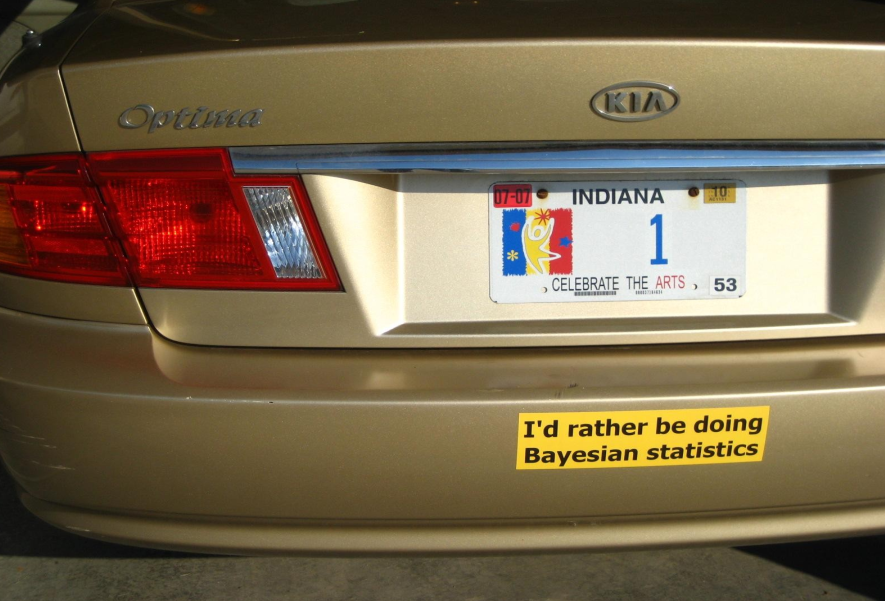
\includegraphics[width=0.6\textwidth]{images/bumper_sticker.png} \\
Credit: John Kruschke
\end{center}

\end{frame}


\begin{frame}
\frametitle{Plan}
\begin{itemize}
\item First we will take a look at an issue involving the use of
probabilities versus probability densities.\pause
\item We will see how to handle multiple data points.\pause
\item Then we will look at {\bf analytic methods}.
\end{itemize}

\end{frame}


\begin{frame}
\frametitle{Computing a Posterior Distribution in R}
Recall the volcano problem, where we had the following assumptions
(prior and sampling distribution respectively) and data,
here written in ``$\sim$'' notation:
\begin{align}
\lambda &\sim \textnormal{Uniform}(0.1, 100) \\
x \given \lambda &\sim \textnormal{Poisson}(\lambda) \\
x &= 20
\end{align}


\end{frame}

\begin{frame}[fragile]
\frametitle{Computing the Posterior Distribution in R}
We represented the uniform prior using the following R vector:
\begin{minted}{r}
lambda = seq(0.1, 100, by=0.1)
prior = rep(1/length(lambda), length(lambda))
\end{minted}
\pause

If we were to make the \mintinline{r}{lambda} grid finer, the probabilities
would get incredibly tiny. It might also be nice to be able to use
\mintinline{r}{dunif()} to make the prior:
\begin{minted}{r}
prior = dunif(lambda, 0.1, 100)
\end{minted}
but this will not sum to 1, because \mintinline{r}{dunif()} returns
probability densities, not probabilities.


\end{frame}


\begin{frame}[fragile]
\frametitle{Probability Densities}
Our new \mintinline{r}{prior} vector created with \mintinline{r}{dunif()}
does not sum to 1, but instead integrates to 1. We can approximate integration
using summation multiplied by the grid spacing to verify this:

\begin{minted}{r}
> lambda = seq(0.1, 100, by=gap)
> prior = dunif(lambda, 0.1, 100)
> sum(gap*prior) # Well, I said it was an approximation!
[1] 1.001001
\end{minted}

We can carry out the entire calculation using densities instead of
probabilities, but every time we do a \mintinline{r}{sum()} we need
to multiply by \mintinline{r}{gap}.

\end{frame}



\begin{frame}[fragile]
\frametitle{Probability Densities}
\begin{minted}{r}
gap = 0.1
lambda = seq(0.1, 100, by=gap)
prior = dunif(lambda, 0.1, 100)
lik = dpois(20, lambda)
h = prior*lik
Z = gap*sum(h)  # Approximately an integral
post = h/Z
plot(lambda, post, type="l")
\end{minted}

\end{frame}


\begin{frame}
\frametitle{Posterior Density}
The values on the $y$-axis are now not tiny, and densities are more appropriately plotted with \mintinline{r}{type="l"}.
\begin{center}
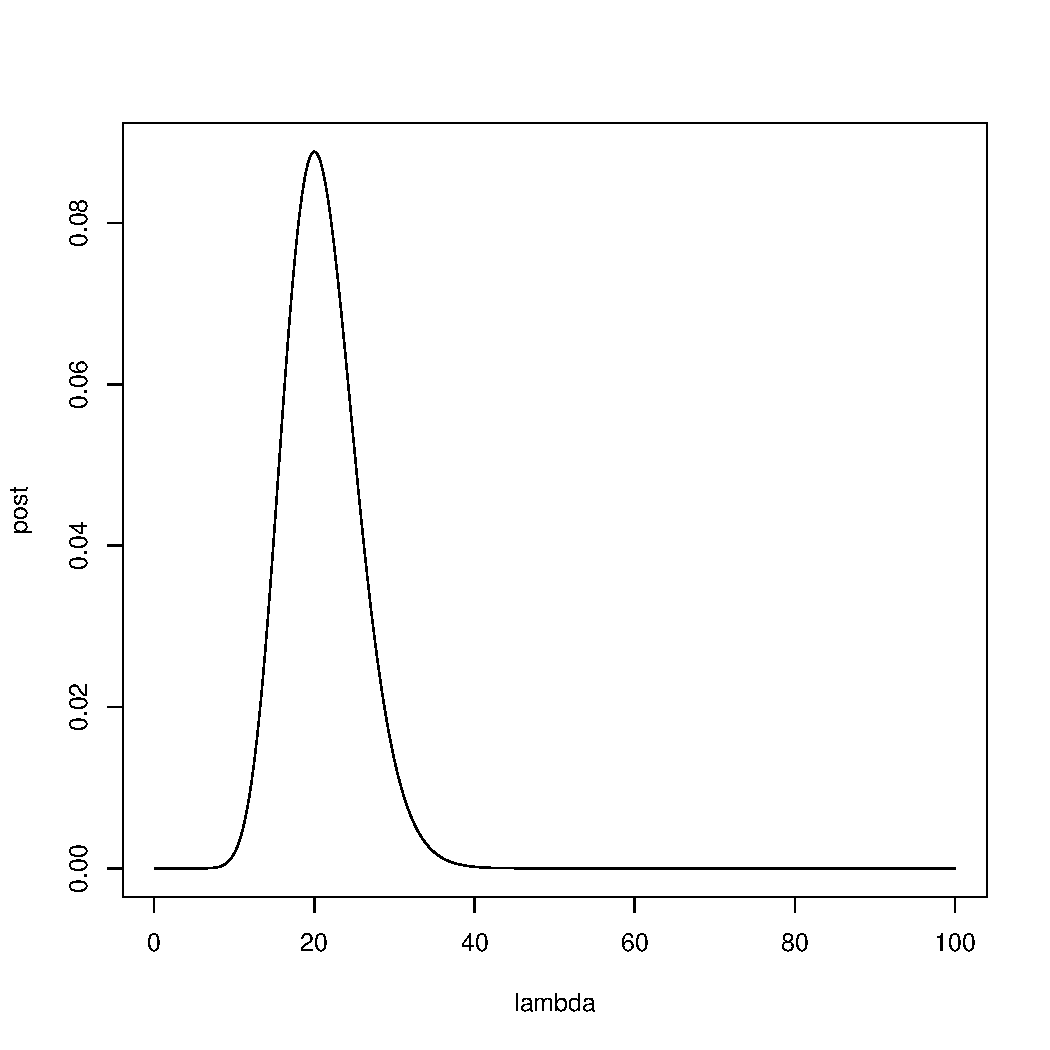
\includegraphics[width=0.35\textwidth]{images/density.pdf}
\end{center}
This method is better if we want to write a prior using
\mintinline{r}{dbeta()} or something (we will see beta distributions soon).

\end{frame}

\begin{frame}[fragile]
\frametitle{Multiple Data Points}
When there are multiple data points, the likelihood is formed from a
{\bf product} of terms, one for each data point.
For example, suppose we had earthquake data for
three non-overlapping 20,000 year periods, and the values were
$\{20, 14, 18\}$.\pause
\begin{minted}{r}
lik = dpois(20, lambda)*dpois(14, lambda)*dpois(18, lambda)
\end{minted}
\pause
When there are many data values, a loop may be needed, and you might
also need to take the log. This will show up in labs.

\end{frame}




\begin{frame}
\frametitle{Parameter Estimation: Analytical Methods}

\begin{center}
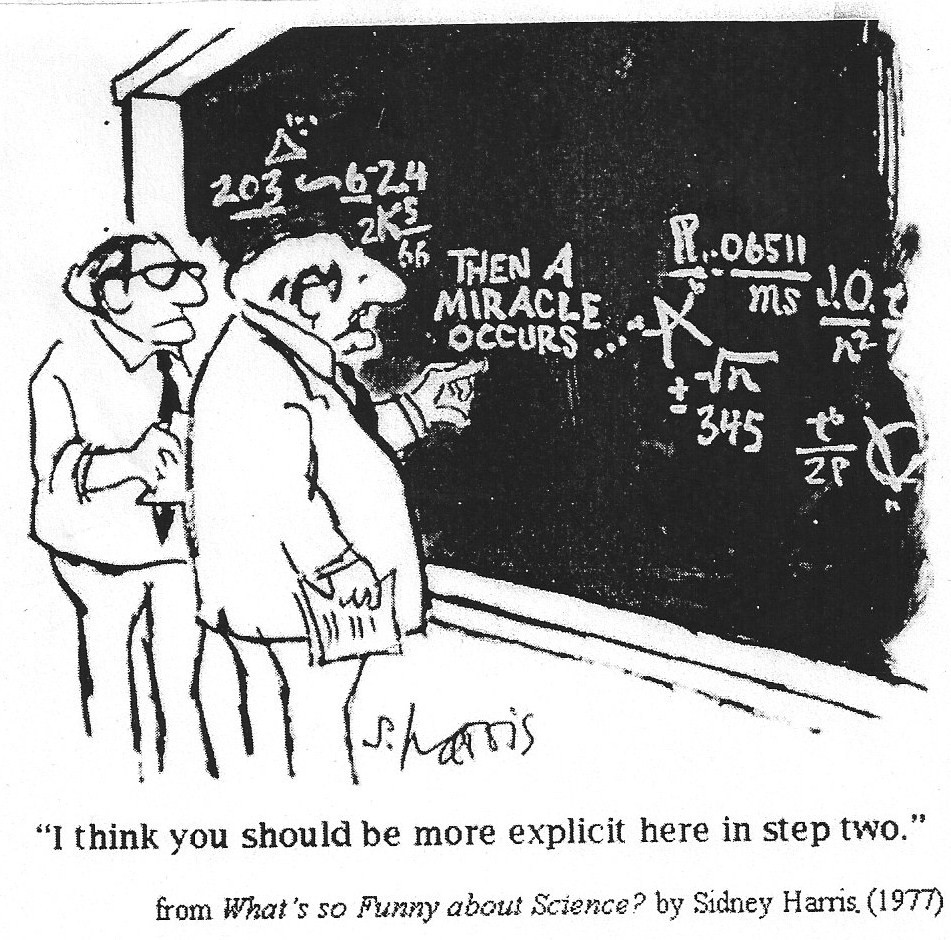
\includegraphics[width=0.6\textwidth]{images/miracle.jpg}
\end{center}

\end{frame}

\begin{frame}
\frametitle{Reminder of Bayes' Rule for Parameter Estimation}

\begin{align}
p(\theta \given x) &= \frac{p(\theta)p(x \given \theta)}{p(x)} \\
p(\theta \given x) &\propto p(\theta)p(x \given \theta) \\
\texttt{posterior} &\propto \texttt{prior} \times \texttt{likelihood}
\end{align}
(notation: $\theta$=parameter, $x$=data)\pause

In analytical methods, we will write down explicit mathematical expressions
for $p(\theta)$ and $p(x \given \theta)$, multiply them, and see what we
get for $p(\theta \given x)$.

\end{frame}


\begin{frame}
\frametitle{Reminder: Election Poll Problem}
We called 10 people and the data was
$\{1, 1, 0, 0, 1, 0, 1, 0, 1, 1\}$. Our likelihood function was
\begin{align}
p(x \given \theta) &= \theta^6(1-\theta)^4.
\end{align}
\pause
In this example, our parameter is actually called $\theta$ and our data may
as well be called $x$. In other problems, it's best to use the symbols
appropriate to the meanings of the parameter(s) and the data.
\end{frame}


\begin{frame}
\frametitle{Uniform Prior}
Let's choose a (continuous) uniform prior between 0 and 1 for $\theta$.
The mathematical expression for this density is
\begin{align}
p(\theta) = \left\{
                \begin{array}{cc}
                1, & 0 \leq \theta \leq 1 \\
                0, & \textnormal{otherwise}.
                \end{array}
            \right.
\end{align}
\pause
However, if we just remember that we're dealing with something between 0 and 1,
we can simply write
\begin{align}
p(\theta) = 1.
\end{align}

\end{frame}

\begin{frame}
\frametitle{Prior Times Likelihood}
By Bayes' rule, the posterior distribution is {\em proportional to}
the prior times the likelihood. We have those now:
\begin{align}
p(\theta \given x) &\propto p(\theta) p(x \given \theta) \\
                   &= 1 \times \theta^6(1-\theta)4 \\
                   &= \theta^6(1-\theta)^4.
\end{align}
\pause
We have the result! However, we need to understand what the distribution
looks like. We can (i) plot the function to see its shape (this will essentially
involve the Bayes' Box steps!) or (ii) we can magically recognise from the
formula what this distribution must be.

\end{frame}


\begin{frame}
\frametitle{Beta Distributions}

\begin{itemize}
\item The {\bf beta distribution} is often used for values that are between 0
and 1.\pause
\item It has two parameters, $\alpha$ and $\beta$, which determine its shape.
For a quantity $x$ with a Beta distribution, we write $x \sim \textnormal{Beta}(\alpha, \beta)$.\pause
\item The probability density equation is
\begin{align}
p(x) &= \frac{1}{\textnormal{Beta}(\alpha, \beta)}
            x^{\alpha - 1}(1-x)^{\beta - 1}
\end{align} \pause
\item We mostly focus on the part that depends on $x$ - the other thing
at the front is just a normalisation constant.
\end{itemize}

\end{frame}

\begin{frame}
\frametitle{Comparing Formulas}

The beta distribution is
\begin{align}
p(x) &= \frac{1}{\textnormal{Beta}(\alpha, \beta)}
            x^{\alpha - 1}(1-x)^{\beta - 1}
\end{align}

and our posterior distribution was
\begin{align}
p(\theta \given x) &\propto \theta^6(1-\theta)^4.
\end{align}\pause
By comparing the two formulas, we see that our posterior is
a Beta$(7, 5)$ distribution. We can write
\begin{align}
\theta \given x &\sim \textnormal{Beta}(7, 5).
\end{align}

\end{frame}

\begin{frame}
\frametitle{Beta Distributions from Wikipedia}

\begin{center}
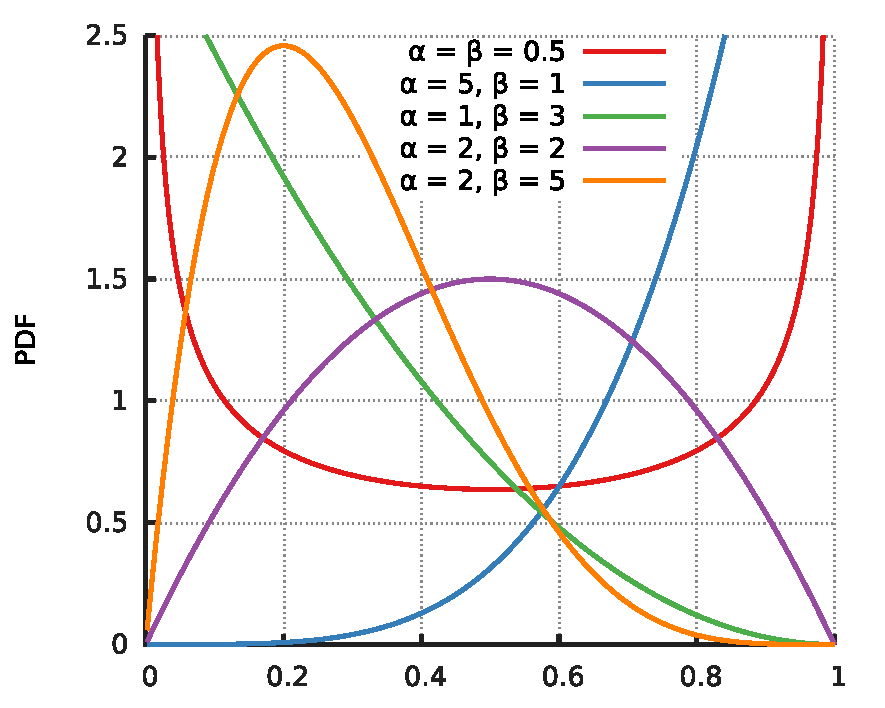
\includegraphics[width=0.6\textwidth]{images/betas.pdf}
\end{center}

\end{frame}

\begin{frame}
\frametitle{Our Beta(7, 5) Posterior}

\begin{center}
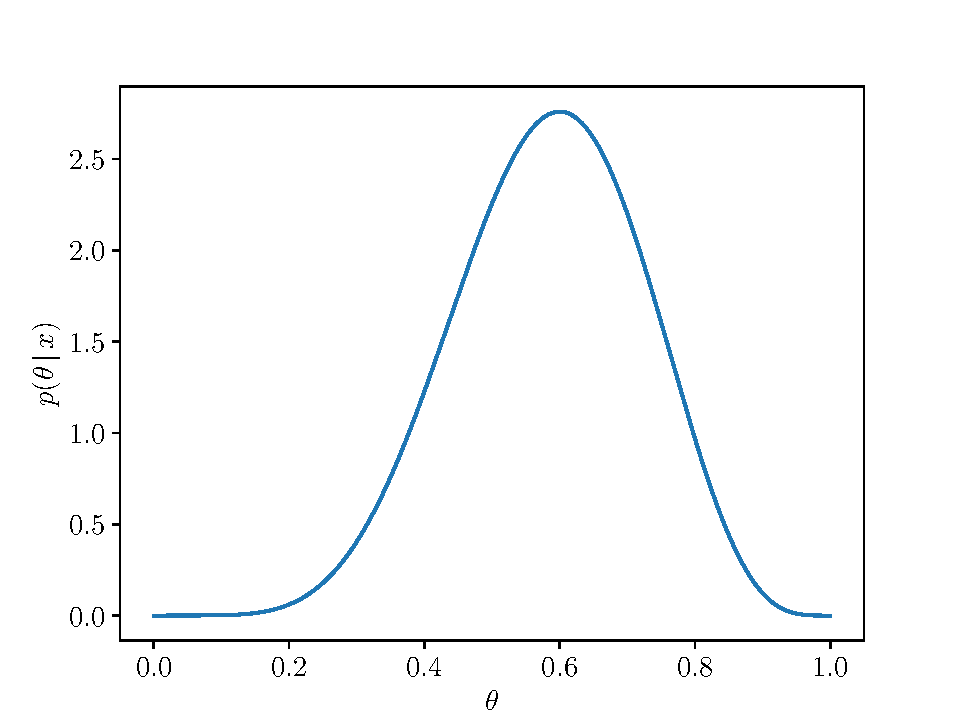
\includegraphics[width=0.6\textwidth]{images/beta_posterior.pdf}
\end{center}

\end{frame}

\begin{frame}
\frametitle{A Special Case}
The Beta(1, 1) distribution is actually the same as a Uniform(0, 1)
distribution. Look at the equation for the probability density:
\begin{align}
p(\theta) &\propto \theta^{\alpha-1}(1-\theta)^{\beta - 1} \\
          &= \theta^{0}(1-\theta)^{0} \\
          &= 1.
\end{align}

\end{frame}



\begin{frame}
\frametitle{Prediction}

\begin{itemize}
\item Let's do a Bayesian prediction using analytical methods. We will be
able to `cheat' instead of doing an integral.\pause
\item What is the probability that the `next' data point is a 1?\pause
\item This will give us Laplace's famous {\bf rule of succession}.
\end{itemize}

\end{frame}

\begin{frame}
\frametitle{Prediction: Bayesian Approach}

\begin{itemize}
\item Step 1: get the posterior distribution for the parameter(s)\pause
\item Step 2: For each possible value of the parameter, compute the probability
you're interested in (e.g., probability that the next data point is a 1).\pause
\item Step 3: Calculate the weighted average of the probabilities from the previous
step, using the posterior distribution for the weights.\pause
\end{itemize}

This procedure is not invented, but is derivable from the rules of
probability theory.

\end{frame}

\begin{frame}
\frametitle{Prediction: Bayesian Approach}
We've done step 1. For step two, consider: if we knew $\theta$, what would
be the probability of the next data point being a 1? Hopefully you can see that
it would simply be $\theta$ itself.\pause

Therefore to do the prediction we ``just'' need to do this integral:
\begin{align}
P(x_{11} = 1 \given x) &= \int_0^1 \theta p(\theta \given x)\, d\theta
\end{align}
where $p(\theta \given x)$ is our Beta$(7, 5)$ posterior. However, someone
has already done it for us!

\end{frame}

\begin{frame}
\frametitle{Expectation of a Beta Distribution}
You might recognise the previous integral as the definition of the
{\bf expectation} of our posterior distribution. Wikipedia has our answer.

\centering
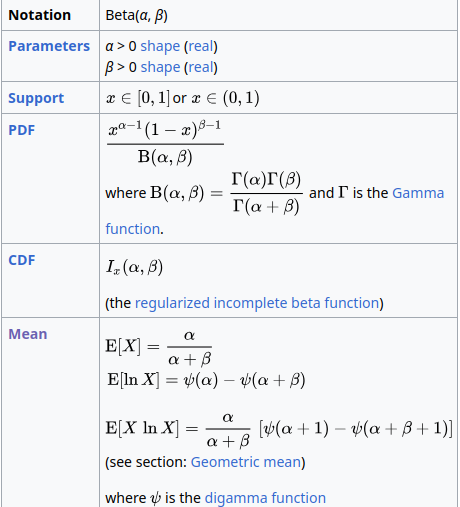
\includegraphics[scale=0.3]{images/wikipedia.png}

\end{frame}


\begin{frame}
\frametitle{Prediction Result}
Let's just use the given result.
\begin{align}
P(x_{11} = 1 \given x) &= \frac{7}{7+5} \\
                       &= 7/12.
\end{align}\pause
In general, for $x$ successes out of $N$ trials and a uniform prior for
$\theta$, the result is {\bf Laplace's rule of succession}:
\begin{align}
P(x_{\rm next} = 1 \given x) &= \frac{x+1}{N+2}.
\end{align}\pause
The result is {\em not} $x/N$, and continues to make sense even with no data
($x=N=0$)!


\end{frame}



\begin{frame}
\frametitle{Beta-Binomial}
Consider the binomial distribution, which is used for the number of successes
$x$ out of $N$ independent ``Bernoulli trials'', with success probability
$\theta$ on each of the trials. The Binomial distribution looks like
\begin{align}
p(x \given \theta) &= \binom{N}{x}\theta^x(1-\theta)^{N-x}.
\end{align}
\pause
If we observe the value of $x$ but want to infer $\theta$, we can derive
the posterior for $\theta$ given $x$. Let's do this now.

\end{frame}


\begin{frame}
\frametitle{Beta-Binomial}
There is a nice relationship between the beta distribution and the binomial
distribution. If the former is the prior for $\theta$ and the latter is the
sampling distribution (which gives the likelihood), then we get a nice
result.\pause
\begin{align}
p(\theta \given x) &\propto p(\theta) p(x \given \theta) \\
    &= \theta^{\alpha-1}(1-\theta)^{\beta-1} \theta^x(1-\theta)^{N-x} \\
    &= \theta^{\alpha+x-1}(1-\theta)^{\beta+N-x-1}
\end{align}
\pause
The posterior is another beta distribution!
\begin{align}
\theta \given x &\sim \textnormal{Beta}(\alpha+x, \beta+N-x)
\end{align}

\end{frame}

\begin{frame}
\frametitle{Rule of Succession}
If we take the expectation, like we did before, to find the predictive
probability of success on the next trial, we get
\begin{align}
\frac{\alpha+x}{\alpha + \beta + N}
\end{align}
as the result. If we choose a uniform prior ($\alpha=\beta=1$)
then we get the rule of succession again, which was
$(x+1)/(N+2)$.

\end{frame}



\begin{frame}
\frametitle{Conjugate Priors}
Beta Prior + Binomial Sampling Distribution $\implies$~
Beta Posterior \\

This is our first example of a {\bf conjugate prior}.
We say that the Beta is the conjugate prior for the Binomial.

\end{frame}


\begin{frame}
\frametitle{Burgers}

\centering
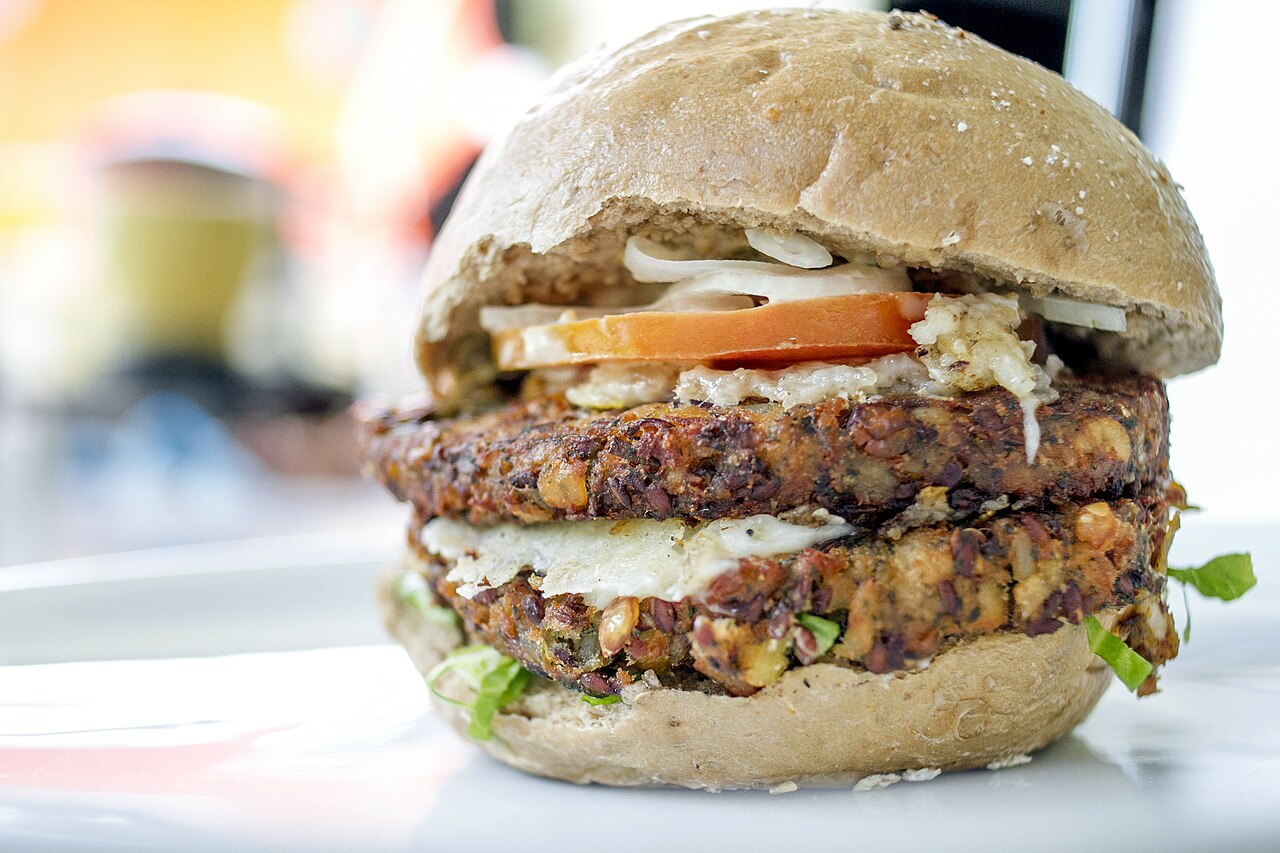
\includegraphics[width=0.7\textwidth]{images/burger.jpg}

By Roee Shpernik, CC BY-SA 4.0, https://commons.wikimedia.org/w/index.php?curid=35019440

\end{frame}


\begin{frame}
\frametitle{Burgers}

\centering
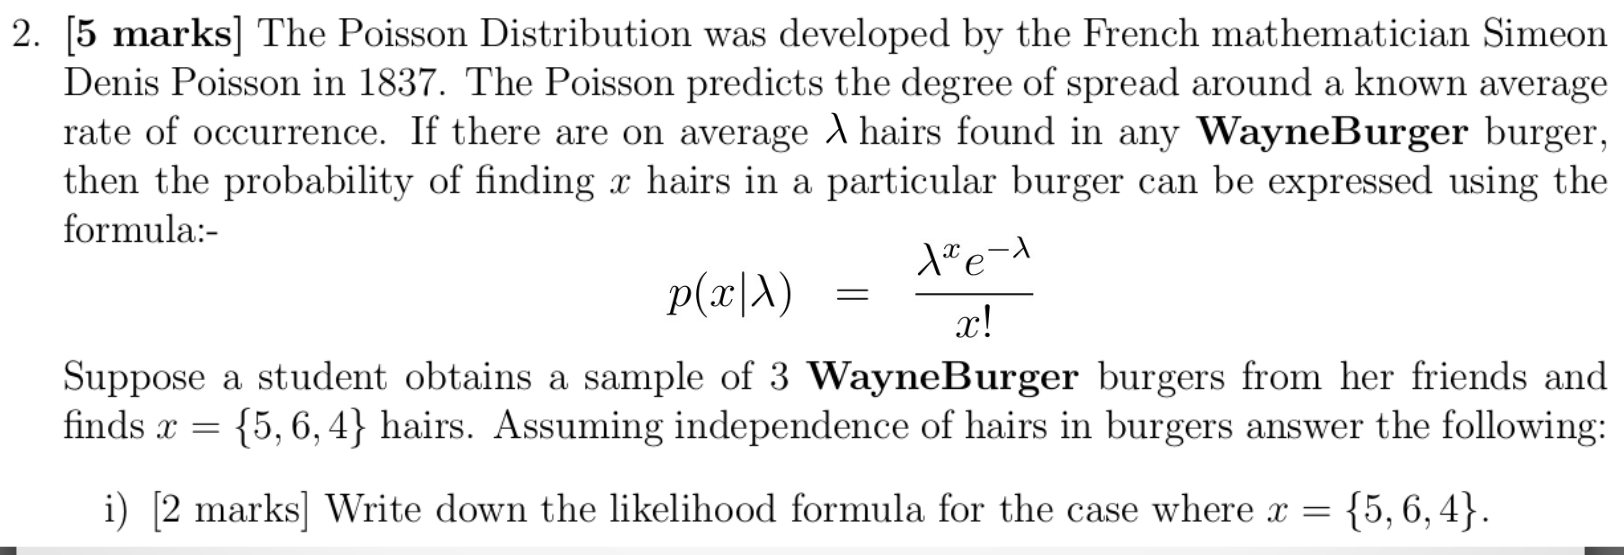
\includegraphics[width=0.7\textwidth]{images/wayneburger.png}

\end{frame}


\begin{frame}
\frametitle{Likelihood}
The likelihood function is formed from the product of the Poisson distribution
three times. Why? It's the probability of getting 5 hairs on the first burger
{\bf and} 6 on the second burger {\bf and} 4 on the third burger --- this is
the product rule in action.\pause
\begin{align}
p(x_1, x_2, x_3 \given \lambda)
    &= \frac{\lambda^{x_1}e^{-\lambda}}{x_1!}
        \frac{\lambda^{x_2}e^{-\lambda}}{x_2!}
        \frac{\lambda^{x_3}e^{-\lambda}}{x_3!} \\
    &\propto 
        \lambda^{x_1+x_2+x_3}e^{-3\lambda} \\
    &= \lambda^{15}e^{-3\lambda}.
\end{align}

\end{frame}


\begin{frame}
\frametitle{Log-Uniform Prior}
The log-uniform prior works nicely here because $\lambda$ must be positive,
and we can imagine being uncertain about the order of magnitude.\pause
\begin{align}
p(\lambda \given x_1, x_2, x_3) &\propto p(\lambda)p(x_1, x_2, x_3 \given \lambda) \\
    &\propto \frac{1}{\lambda} \lambda^{15}e^{-3\lambda} \\
    &= \lambda^{14}e^{-3\lambda}.
\end{align}
\pause
What distribution is this?

\end{frame}


\begin{frame}
\frametitle{Gamma Distribution}
Gamma distributions are used for positive quantities, and the
probability density function looks like this, with a polynomial factor
and an exponential factor:
\begin{align}
p(x \given \alpha, \beta)
    &= \frac{\lambda^{\alpha}}{\Gamma(\alpha)}
            x^{\alpha-1}e^{-\beta x}.
\end{align}
\pause
As before, we can just focus on the part that depends on $x$ (which corresponds
to $\lambda$ on the previous slide). By matching terms we see that we have
\begin{align}
\lambda \given x_1, x_2, x_3 \sim \textnormal{Gamma}(15, 3).
\end{align}

\end{frame}


\begin{frame}
\frametitle{Our Gamma(15, 3) Posterior}

\centering
\includegraphics[width=0.6\textwidth]{images/gamma_posterior.pdf}

\end{frame}


\begin{frame}
\frametitle{Gamma Distributions from Wikipedia}
\centering
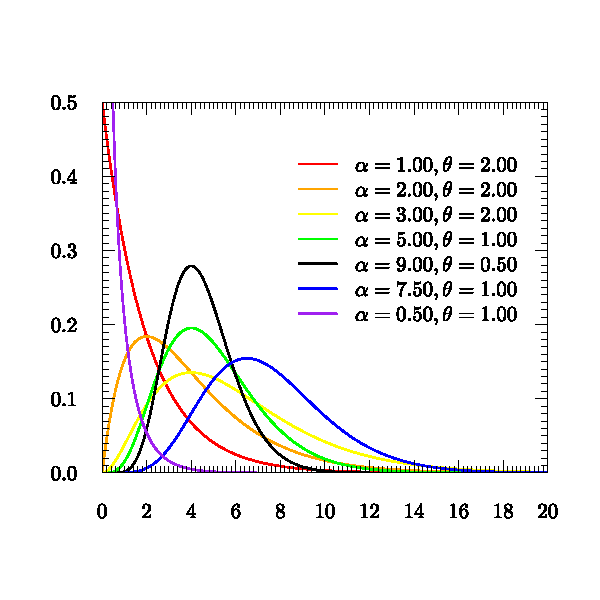
\includegraphics[width=0.7\textwidth]{images/gammas.pdf}

\end{frame}


\begin{frame}
\frametitle{Gamma-Poisson}

The gamma distribution is actually the conjugate prior for the Poisson distribution. This means:

Gamma Prior + Poisson Sampling Distribution $\implies$~Gamma Posterior.

Let's derive this now.


\end{frame}


\begin{frame}
\frametitle{Gamma-Poisson}
Suppose we have $x_1, x_2, ..., x_N$ and our sampling distribution for these
is Poisson with parameter/mean $\lambda$. We use a gamma prior for $\lambda$.
\pause
\begin{align}
p(\lambda \given x_1, ..., x_N)
    &\propto p(\lambda)p(x_1, ..., x_N \given \lambda) \\
    &\propto \lambda^{\alpha-1}e^{-\beta \lambda}
            \prod_{i=1}^N \lambda^{x_1}e^{-\lambda} \\
    &= \lambda^{\alpha + \sum_{i=1}^N x_i}e^{-(\beta + N)\lambda}
\end{align}
Therefore, the posterior is
\begin{align}
\lambda \given x_1, ..., x_N &\sim
    \textnormal{Gamma}\left(\alpha + \sum_{i=1}^N x_i, \beta + N\right).
\end{align}



\end{frame}


\begin{frame}
\frametitle{Normal-Normal}
\begin{itemize}
\item The other famous conjugate prior is the normal-normal. However, this is a bit
messy, so I prefer to skip it in STATS 331 (it is studied in STATS 731).\pause
\item It also assumes the $\sigma$ of the normal distribution is known, which
is unrealistic.\pause
\item If you assume $\sigma$ is unknown, you can derive a posterior distribution
which is a Student-$t$ distribution.
\end{itemize}

\end{frame}


\begin{frame}
\frametitle{Analytical Methods: Pros and Cons}

{\bf Pros}
\begin{itemize}
\item Answers are exact with no need for approximate grids.\pause
\item The posterior distribution is often easy to use to compute
    predictions or summaries (we will look at summaries soon).
\end{itemize}
\pause
{\bf Cons}
\begin{itemize}
\item The trick of `recognising' the posterior distribution from its formula
is only possible in a few special cases.
\end{itemize}


\end{frame}



\begin{frame}
\frametitle{What I Expect of You}
In STATS 331 I expect you to be able to work with the Binomial and
Poisson situations and their respective conjugate priors.

\end{frame}



\end{document}

